\let\workinterval\relax
\let\ckpttime\relax
\let\txdelay\relax
\let\msgtime\relax
\let\minheight\relax
\newcommand{\workinterval}{1.25cm}
\newcommand{\ckpttime}{0.625cm}
\newcommand{\txdelay}{2.0mm}
\newcommand{\msgtime}{\workinterval+\txdelay}
\newcommand{\minheight}{0.5cm}
\usetikzlibrary{positioning}

\tikzstyle{position}=[fill=none,text=white,draw=none]
\tikzstyle{proc}=[fill=none,text=black,draw=none,shape=rectangle]
\tikzstyle{origtotal}=[fill=none,text=black,draw=black,shape=rectangle,
                       minimum width=3*\workinterval+2*\txdelay,
                       minimum height=\minheight]
\tikzstyle{coordtotal}=[fill=none,text=black,draw=black,shape=rectangle,
                        minimum width=3*\workinterval+\ckpttime+2*\txdelay,
                        minimum height=\minheight]
\tikzstyle{uncoordtotal}=[fill=none,text=black,draw=black,shape=rectangle,
                          minimum width=3*\workinterval+2*\ckpttime+2*\txdelay,
                          minimum height=\minheight]
\tikzstyle{ckpt}=[fill=black,text=white,draw=none,shape=rectangle,
                  minimum width=\ckpttime,minimum height=\minheight]
\tikzstyle{stall}=[fill=black!20,text=white,draw=black,shape=rectangle,
                   minimum height=\minheight]

\begin{figure*}[bt]
\centering{
\subfloat[without CE activity]{
\resizebox{0.25\textwidth}{!}{
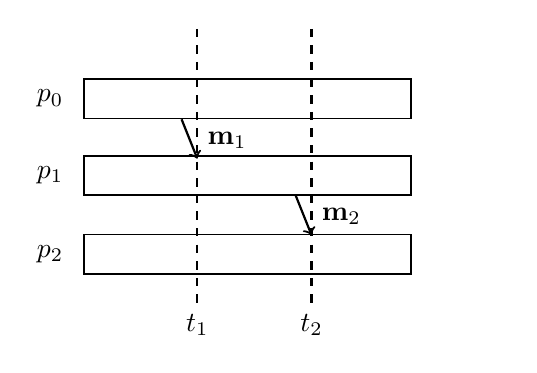
\begin{tikzpicture}[semithick]

\node [proc] (p0) {$p_0$};
\node [position, right= 0.125cm of p0, minimum width=3*\workinterval+2*\ckpttime+2*\txdelay] (n0) {};
\node [origtotal, right= 0.125cm of p0]  (v1) {};
\node [position, right= \msgtime of v1.north west ]  (v2) {};
\node [position, right= \msgtime of v2.west ]  (v4) {};

\node [proc, below = 5mm of p0] (p1) {$p_1$};
\node [origtotal, right= 0.125cm of p1]  (v5) {};
\node [position, right= \msgtime of v5.west ]  (v6) {};
\node [position, right= \workinterval of v6.south west ]  (v8) {};

\node [proc, below of=p1] (p2) {$p_2$};
\node [origtotal, right= 0.125cm of p2]  (v9) {};
\node [position, right= \msgtime of v9.west ]  (v10) {};
\node [position, right= \msgtime of v10.west ]  (v11) {};

\draw [->, thick] (v1.south west) ++(\workinterval,0) -- ++(\txdelay, -5.00mm) 
      node[above right] {$\mathbf{m}_1$};
\draw [->, thick] (v8.south west) -- ++(\txdelay, -5.00mm) node[above right] {$\mathbf{m}_2$};

\draw [thick, dashed] (v2.north west) ++(0.0cm, 5.0mm) -- (v10.south west) -- ++(0, -5.0mm) node[below] {$t_1$};
\draw [thick, dashed] (v4.north west) ++(0.0cm, 5.0mm) -- (v11.south west) -- ++(0, -5.0mm) node[below] {$t_2$};
\end{tikzpicture} 
}\label{subfig:no_ckpt}
}
%
%
%\subfigure[uncoordinated checkpointing]{
\subfloat[with local CE activity delays]{
\resizebox{0.25\textwidth}{!}{
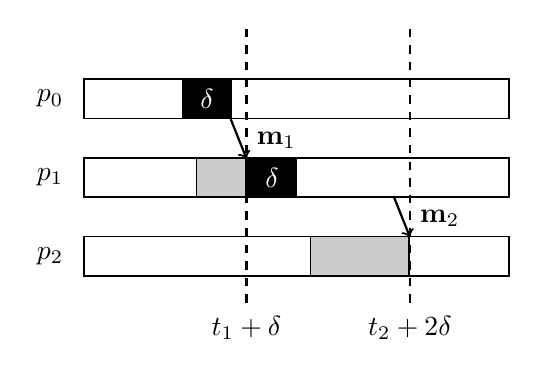
\begin{tikzpicture}[semithick]

\node [proc] (p0) {$p_0$};
\node [uncoordtotal, right= 0.125cm of p0]  (v1) {};
\node [position, right= \msgtime+\ckpttime of v1.north west ]  (v2) {};
\node [ckpt, right= \workinterval of v1.west ]  (v3) {$\delta$};
\node [position, right= \msgtime+\ckpttime of v2.west ]  (v4) {};

\node [proc, below of=p0] (p1) {$p_1$};
\node [uncoordtotal, right= 0.125cm of p1]  (v5) {};
\node [position, right= \msgtime+\ckpttime of v5.west ]  (v6) {};
\node [stall, minimum width=\ckpttime, left= 0.0cm of v6.west ]  (v7) {};
\node [ckpt, right= 0.00cm of v6.west ]  (v7) {$\delta$};
\node [position, right= \workinterval+\ckpttime of v6.south west ]  (v8) {};

\node [proc, below of=p1] (p2) {$p_2$};
\node [uncoordtotal, right= 0.125cm of p2]  (v9) {};
\node [position, right= \msgtime+\ckpttime of v9.west ]  (v10) {};
\node [position, right= \msgtime+\ckpttime of v10.west ]  (v11) {};
\node [stall, minimum width=2*\ckpttime, left= 0.00cm of v11.west ]  (v12) {};

\draw [->, thick] (v1.south west) ++(\workinterval+\ckpttime,0) -- ++(\txdelay, -5.00mm) 
      node[above right] {$\mathbf{m}_1$};
\draw [->, thick] (v8.south west) -- ++(2.0mm, -5.00mm) node[above right] {$\mathbf{m}_2$};

\draw [thick, dashed] (v2.north west) ++(0.0cm, 5.0mm) -- (v10.south west) -- ++(0, -5.0mm) node[below] {$t_1+\delta$};
\draw [thick, dashed] (v4.north west) ++(0.0cm, 5.0mm) -- (v11.south west) -- ++(0, -5.0mm) node[below] {$t_2+2\delta$};
\end{tikzpicture} 
}\label{subfig:uncoord_ckpt}
}
}
\caption{
        Example of how delays introduced by local correctable error (CE)
        activities may propagate along application communication dependencies.
        The processes $p_1$, $p_2$, and $p_3$ exchange two messages $m_1$ and
        $m_2$ in each of the three scenarios. The black regions marked with a
        white $\delta$ denote the execution of CE mitigation activities.  The
        grey regions denote periods in which the execution of a process is
        stalled due to an unsatisfied communication dependency.
}\label{fig:propagation}
\end{figure*}
